\documentclass[11pt]{book}

% Packages for Figures:
\ifx\pdftexversion\undefined
    \usepackage[dvips]{graphicx}
\else
    \usepackage[pdftex]{graphicx}
    \usepackage{epstopdf}
    \epstopdfsetup{suffix=}
\fi

% Packages for displaying code:
\usepackage{listings}
\usepackage{textcomp}
\usepackage{color}

% Color settings used in the code below:
\definecolor{dkgreen}{rgb}{0,0.6,0}
\definecolor{gray}{rgb}{0.5,0.5,0.5}
\definecolor{mauve}{rgb}{0.58,0,0.82}

% Settings for the formatting of the code on display:
\lstset{frame=tb,
  language=R,
  aboveskip=3mm,
  belowskip=3mm,
  showstringspaces=false,
  columns=flexible,
  basicstyle={\small\ttfamily},
  numbers=none,
  numberstyle=\tiny\color{gray},
  keywordstyle=\color{blue},
  commentstyle=\color{dkgreen},
  stringstyle=\color{mauve},
  breaklines=true,
  breakatwhitespace=true,
  tabsize=3
}


\begin{document}


\section*{Histogram of a Randomly Generated Variable}

We ran the following commands in R.

\begin{lstlisting}[language=R]

\input{Code/my_script.R}
    
\end{lstlisting}


The histogram in Figure \ref{fig:example} shows the result of these commands.

\begin{figure}
\centering
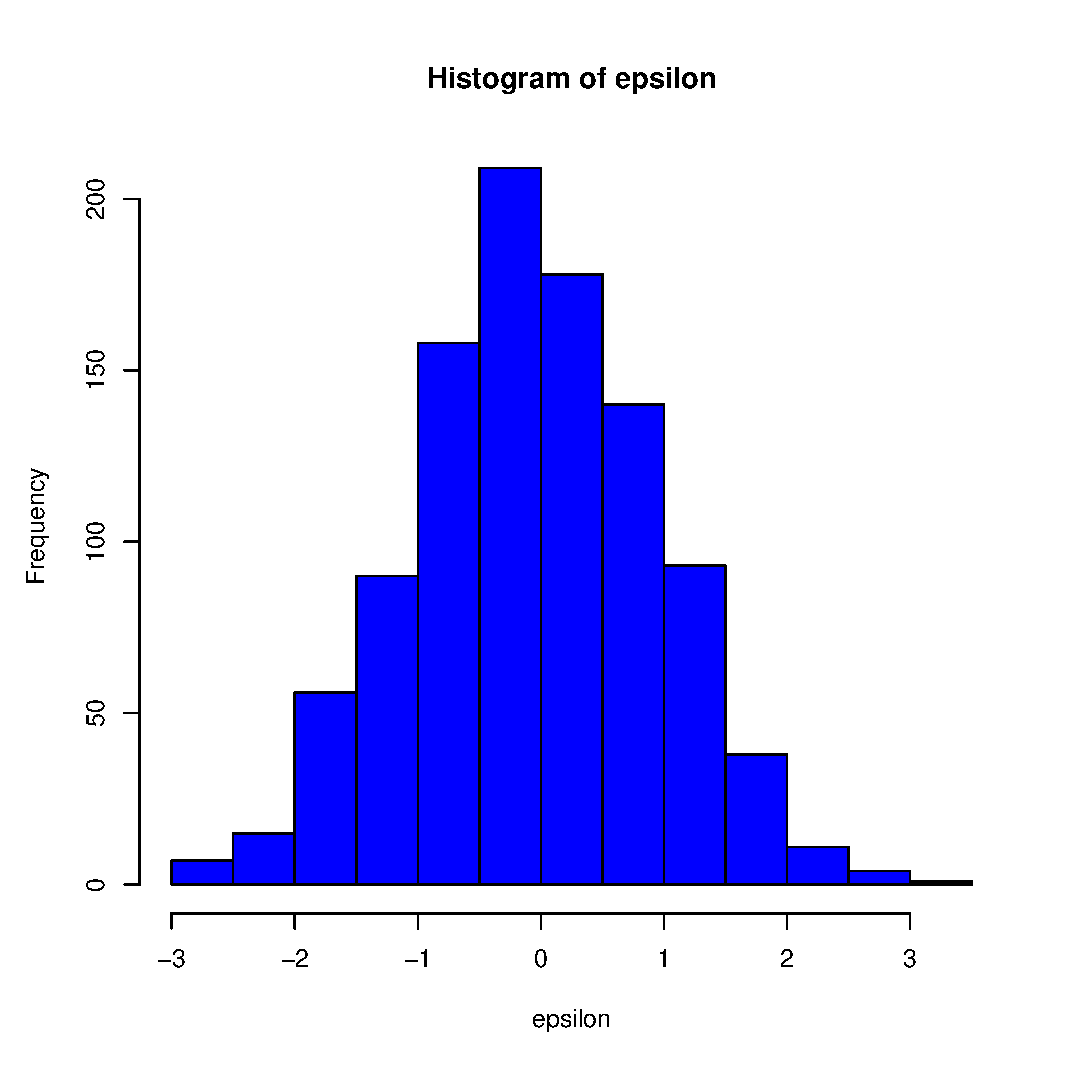
\includegraphics[width=\textwidth]{Figures/name_of_figure.eps}
\caption{Caption Goes Here}
\label{fig:example}
\end{figure}


\end{document}
